\section{Introduzione}
In questa fase, forniremo le basi dei concetti teorici e degli strumenti utilizzati nel corso del progetto. Vedremo in dettaglio come sia stato impostato l'ambiente di sviluppo e come sia stato affrontato il problema in analisi.

\subsection{Richieste}
La società fittizia STECCAPARAPETUTTI S.R.L. richiede l'analisi dei dati delle vendite del sistema di contabilità dell'anno precedente. I dati sono contenuti in un file CSV strutturato in modo omogeneo. L'analisi richiede il calcolo della media e della varianza delle vendite per ogni mese di ogni anno, l'identificazione del mese di ogni anno con la maggiore e minore vendita. Per ogni lavoro, è necessaria la documentazione dell'implementazione in R e dell'implementazione del paradigma MapReduce di Hadoop. Il risultato finale deve essere presentato sotto forma di un rapporto completo.

\subsection{Introduzione all’ambiente}
\subsubsection{MapReduce}
L'algoritmo MapReduce è un modello di programmazione e un'infrastruttura di elaborazione distribuita utilizzata per elaborare e generare informazioni da enormi quantità di dati in modo efficiente, sicuro e scalabile. È stato introdotto da Google\cite{mapReduceGoogle} e ha giocato un ruolo fondamentale nel campo del data processing su larga scala.

L'idea alla base di MapReduce è suddividere un grande task di elaborazione dei dati in due fasi principali: la fase di "map" e la fase di "reduce" (più una fase intermedia totalmente automatizzata):

\begin{itemize}
    \item Durante la fase di MapReduce, i dati di input vengono suddivisi in piccoli frammenti e passati a un insieme di processi paralleli chiamati "mapper". Ogni mapper esegue una funzione di mappatura definita dall'utente che prende in ingresso un dato e produce una serie di coppie chiave-valore intermedie. Queste coppie rappresentano il risultato dell'elaborazione dei dati da parte dei mapper.
    \item Dopo la fase di map, il sistema raggruppa le coppie chiave-valore in base alle chiavi e le ordina nella fase di Shuffle e Sort. Questo è un passaggio cruciale poiché consente ai dati correlati di essere inviati allo stesso processo di "reduce".
    \item In questa fase, il sistema assegna le coppie chiave-valore raggruppate ai processi "reducer". Ogni processo reducer esegue una funzione di riduzione definita dall'utente che agisce sulle coppie chiave-valore correlate e produce i risultati finali dell'elaborazione.
\end{itemize}

\begin{figure}[H]
    \centering
    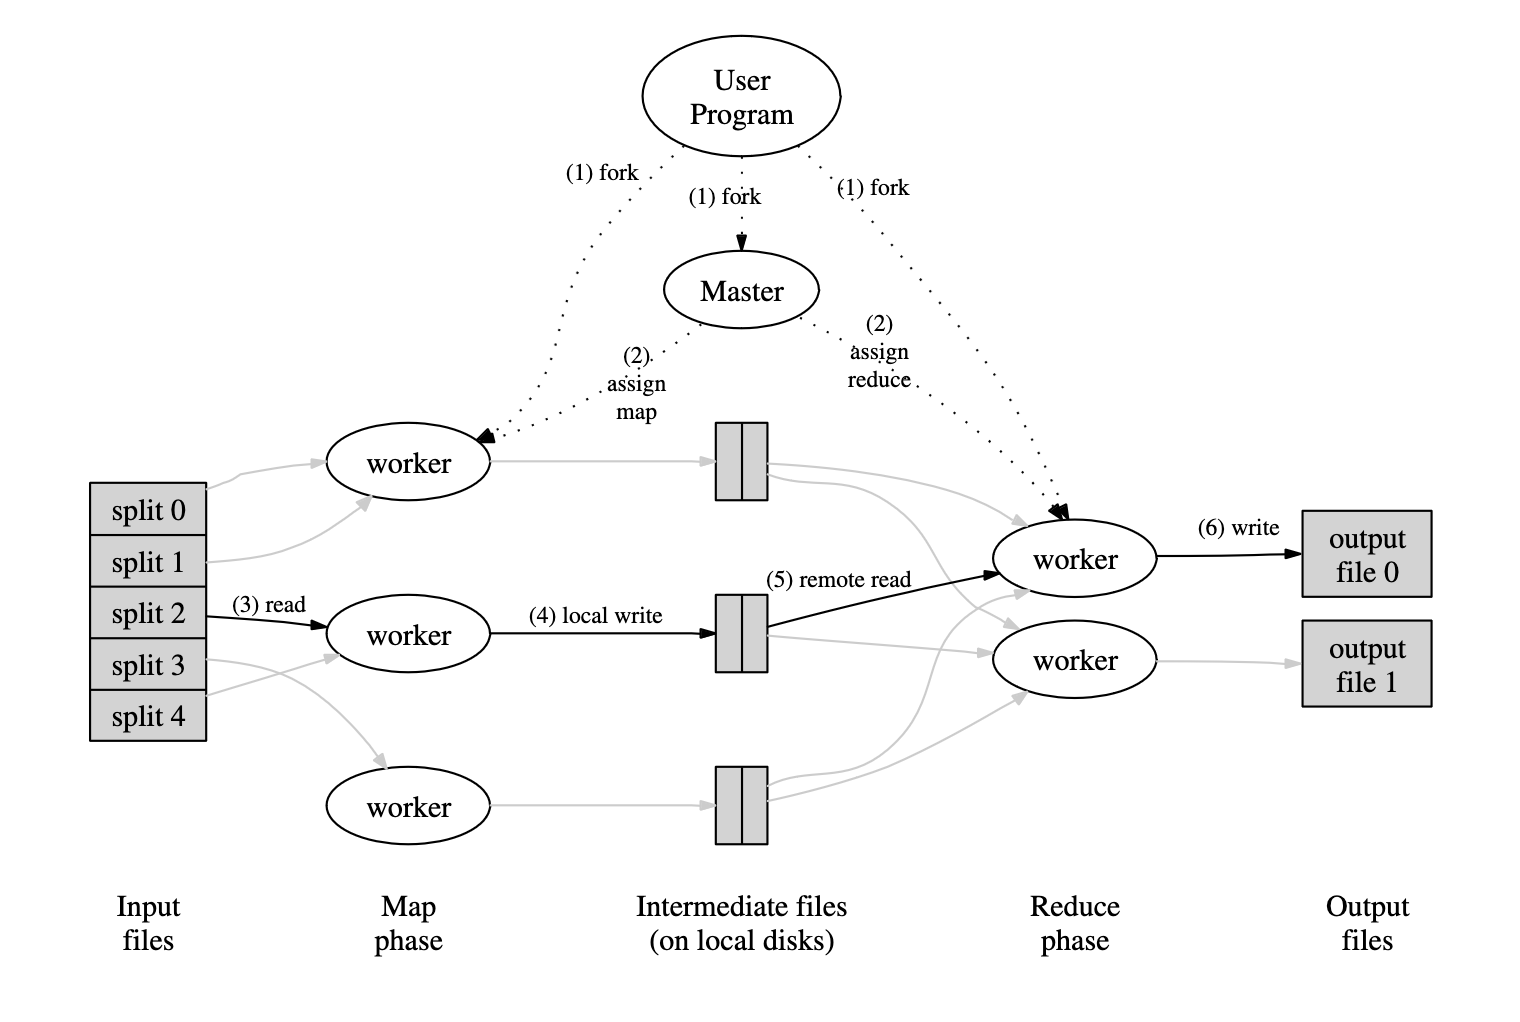
\includegraphics[scale=.4]{img/mapReduceGoogle.png}
    \caption{Schema del processo di MapReduce tratto dal paper di Google}
    \label{mapReduceGoogle}
\end{figure}
L'obiettivo di MapReduce è la parallelizzazione e la distribuzione del carico di lavoro su un cluster di computer, consentendo di elaborare grandi quantità di dati in modo più veloce ed efficiente rispetto a un approccio sequenziale tradizionale. Questo modello di programmazione nasconde molti dettagli complessi dell'elaborazione distribuita, semplificando la creazione di applicazioni che possono sfruttare l'elaborazione su larga scala senza doversi preoccupare delle questioni di basso livello.

Questo ha portato negli anni alla nascita di tecnologie e framework, come Apache Hadoop e Apache Spark, che forniscono funzionalità di MapReduce ma più avanzate e versatili per l'elaborazione distribuita dei dati.

\subsubsection{Hadoop}
Apache Hadoop è un framework open-source sviluppato per consentire l'elaborazione distribuita di grandi quantità di dati su cluster di computer. È basato sulla paper originale di Google su MapReduce e il file system distribuito Google File System (GFS). Hadoop è progettato per gestire l'elaborazione di dati in parallelo su macchine commodity (hardware relativamente economico e accessibile).

Il cuore di Hadoop\cite{ApacheHadoopSite} è composto da due componenti principali: Hadoop Distributed File System (HDFS) e il framework di elaborazione MapReduce.

\begin{enumerate}
    \item Hadoop Distributed File System (HDFS): HDFS è il sistema di archiviazione distribuito di Hadoop. Si basa su un modello di architettura master-slave in cui un nodo master, chiamato "NameNode", gestisce i metadati del file system e tiene traccia di dove sono archiviati i dati. I nodi slave, chiamati "DataNode", contengono i blocchi di dati reali. I dati vengono suddivisi in blocchi e replicati su vari DataNode per garantire la disponibilità e l'affidabilità.
    \begin{figure}[H]
        \centering
        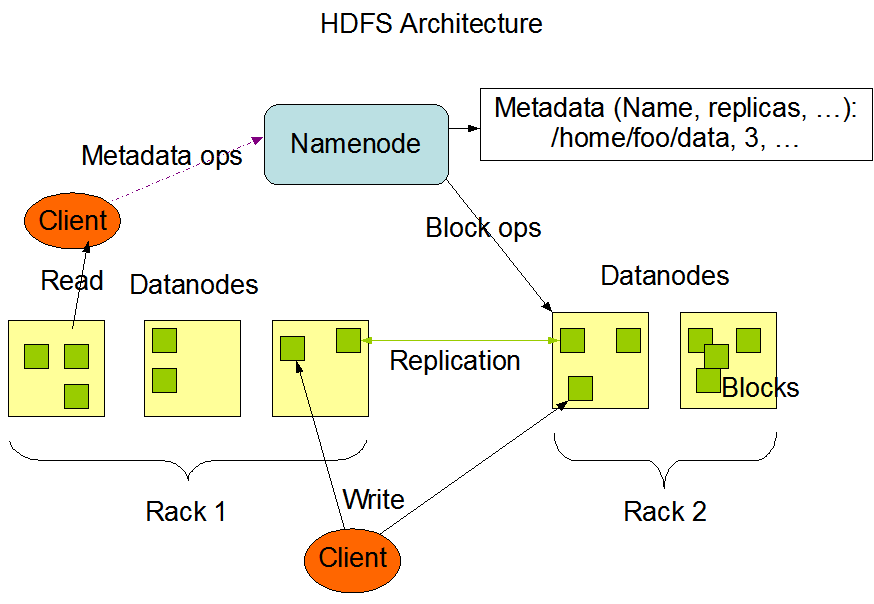
\includegraphics[scale=.4]{img/hdfsarchitecture.png}
        \caption{Schema dell'architettura HDFS tratto dal sito di Hadoop}
        \label{hdfsarchitecture}
    \end{figure}
    \item MapReduce: Come descritto in precedenza, MapReduce è un modello di programmazione per l'elaborazione distribuita. Hadoop implementa questo modello consentendo agli sviluppatori di scrivere programmi MapReduce per l'elaborazione dei dati su cluster. Il framework si occupa della distribuzione delle attività di map e reduce su diversi nodi del cluster, dell'ordinamento e dell'aggregazione dei risultati intermedi e della gestione dei fallimenti dei nodi.
\end{enumerate}

I punti di forza di Hadoop includono la scalabilità orizzontale, la tolleranza ai guasti, l'economia hardware, l'ecosistema di strumenti, l'elaborazione su larga scala, la flessibilità nei tipi di dati e l'elaborazione di dati grezzi. Tuttavia, Hadoop ha anche alcuni svantaggi come la complessità nella configurazione e gestione di un cluster, la latenza, la memoria limitata, l'approccio orientato ai batch, la complessità della programmazione e la concorrenza da parte di framework alternativi come Apache Spark.
\subsubsection{R e RStudio}
R è un linguaggio di programmazione e un ambiente di sviluppo utilizzati principalmente per l’analisi statistica e la visualizzazione dei dati, progettato per lavorare con dataset di varie dimensioni e complessità. Offre un'ampia gamma di funzioni statistiche, algoritmi e pacchetti per l'analisi dei dati, il machine learning, l'analisi delle serie temporali e altro ancora. Inoltre, R fornisce potenti strumenti di visualizzazione che consentono di creare grafici e grafici per rappresentare i dati in modo efficace.

RStudio è un ambiente di sviluppo integrato (IDE) progettato specificamente per lavorare con il linguaggio di programmazione R. Come R\cite{installR} anche RStudio\cite{installRstudio} è un progetto open source che ha lo scopo di offrire un'interfaccia utente intuitiva e ben organizzata che semplifica la scrittura del codice R, l'analisi dei dati e la creazione di visualizzazioni.

\subsubsection{Python}
Python\cite{installPython} è un linguaggio di programmazione che ha catturato l'attenzione di sviluppatori di tutto il mondo grazie alla sua natura versatile e alla sua sintassi chiara e leggibile. Creato da Guido van Rossum\cite{wikiPython} e presentato nel lontano 1991, Python ha continuato a guadagnare popolarità nel corso degli anni, diventando uno dei linguaggi più utilizzati e apprezzati nella comunità dello sviluppo software.

Ciò che distingue Python è il suo approccio alla scrittura del codice. La sua sintassi è strutturata in modo simile al linguaggio naturale, rendendo il codice scritto in Python quasi come una conversazione tra lo sviluppatore e la macchina. Questa semplicità e leggibilità non solo agevolano la creazione del codice, ma anche la comprensione dello stesso da parte di altri sviluppatori, favorendo una collaborazione più agevole.

Python (come anche R) è un linguaggio interpretato, il che significa che non richiede una fase di compilazione separata. Questo aspetto favorisce un approccio di sviluppo più rapido e interattivo, consentendo agli sviluppatori di scrivere e testare il codice in modo immediato, senza dover attendere processi di compilazione lungo.
\subsubsection{Tool Javascript-html per MapReduce}
Per evitare possibili complicazioni dovute alla configurazione di Hadoop, il Professore Daniele Pirrone ha creato uno script web chiamato "Tool MapReduce". Questo strumento consente di simulare un programma MapReduce attraverso un browser generico su Internet.

Lo strumento è sviluppato in Javascript con interfaccia HTML, rendendolo compatibile con i principali sistemi operativi e browser. Il codice è rilasciato sotto licenza GPL.

Lo strumento è semplicemente uno strumento didattico di supporto per gli studenti e quindi:
\begin{itemize}
    \item Consente l'utilizzo di file di input che sono limitati in dimensione alla capacità del computer su cui viene eseguito.
    \item Accetta solo file di testo come input (la maggior parte dei quali hanno un'estensione .txt).
    \item Simula il paradigma di programmazione parallela MapReduce, ma in realtà funziona in modalità stand-alone, non distribuita.
\end{itemize}


\subsection{Preparazione dell’ambiente}
Affrontiamo ora il processo di installazione e configurazione dell'ambiente di sviluppo su macchina virtuale, che si è rivelato necessario per una corretta comunicazione tra Hadoop, RStudio e Python.

Le principali motivazioni di questa scelta risiedono nel fatto che i packages di RHadoop per una corretta comunicazione tra RStudio e Hadoop non sono aggiornati alle ultime versioni \footnote{l’ultima release di RHadoop risale al 2015}.

La scelta di utilizzare la versione di Hadoop all'interno di una macchina virtuale anziché installarla direttamente sul sistema locale è stata influenzata da problematiche di gestione del DFS estendendo tutto il disco a HDFS andando quindi a creare conflitti.

Sfruttando il contesto isolato che offre la virtualizzazione si ha potuti sperimentare con un approccio trial and error diverse configurazioni che permettessero il corretto funzionamento di tutte le componenti. Sono state così fatte scelte specifiche per quanto riguarda le versioni dle sistema operativo e dei software da utilizzare, tenendo conto della compatibilità tra di essi e delle raccomandazioni della comunità.

Si è scelto Virtualbox come sistema di virtualizzazione in quanto software open source di ampia distribuzione.
\subsubsection{Preparazione dell'ambiente virtuale}
Il primo passo è stato creare una nuova macchina virtuale su VirtualBox dal sistema host assegnando risorse hardware adeguate.
\begin{table}[ht]
\centering
\begin{tabularx}{\textwidth}{|X|X|X|X|X|}
\hline
Ruolo & Sistema Operativo & CPU & RAM & Spazio su disco \\
\hline
Host & macOS Ventura 13.4 & 2.3 GHz Intel Core i5 dual-core & 16 GB 2133 MHz LPDDR3 & 500 GB \\
\hline
VM & Ubuntu 16.04 & 1 CPU & 4 GB & 80 GB \\
\hline
\end{tabularx}
\caption{Specifiche di sistema}
\label{tab:specifiche}
\end{table}
    
È stata scelta una distribuzione Linux come sistema operativo ospite per sfruttare la flessibilità e le prestazioni offerte da questa piattaforma open source. Essendo infatti Apache Hadoop un sistema utilizzato principalmente lato server, la sua implementazione più diffusa e stabile è in ambiente UNIX.
\subsubsection{Installazione di Hadoop}
Per garanzie di compatibilità si è scelto la versione 2.6.5 di Apache Hadoop, andandolo a configurare in modalità Single Node Cluster. Successivamente si è anche cercato di aggiungere nodi al cluster ma con risultati poco stabili.\footnote{In una configurazione iniziale si era utilizzata sia una soluzione "fisica" con due Raspberry Pi 3 Model B come nodi dati, sia macchine virtuali Ubuntu Server 22.04. Entrambe le soluzioni hanno presentato problematiche, quindi si è preferito tornare alla configurazione Single Node.}
\subsubsection{Integrazione di RStudio}
L'integrazione di RStudio è stata relativamente più semplice utilizzando la versione 1.0.153 del 2017 e versione di R 3.2.3 che ha permesso una installazione delle librerie di RHadoop senza conflitti.
\subsubsection{Configurazione di Python}
La configurazione di Python presente già nel sistema operativo offre le versioni 2.7 e 3.5.2 con i relativi comandi python e python3. L’unica configurazione necessaria è stata l’intallazione del gestore di pacchetti Python “pip” per l’installazione delle librerie utilizzate poi negli script.
\subsubsection{Conclusione configurazione}
L'installazione e la configurazione dell'ambiente di sviluppo su VirtualBox con Hadoop, RStudio e Python hanno richiesto un approccio meticoloso e la risoluzione di diverse sfide tecniche. Le scelte fatte durante il processo sono state guidate dalla necessità di garantire l'integrazione corretta dei componenti e l'ottimizzazione delle risorse disponibili.


